\chapter{Estado del arte y marco teórico}
\label{chap:estado_arte}

\lettrine{P}{ara} comprender adecuadamente las decisiones arquitectónicas y técnicas tomadas en este proyecto, es fundamental contextualizar los conceptos teóricos subyacentes. Este capítulo describe los fundamentos de la Inteligencia de Negocios y las herramientas ETL que sustentan el Datamart desarrollado.

\section{Inteligencia de negocios y data warehousing}
La Inteligencia de Negocios (\textit{business intelligence} o BI) comprende el conjunto de metodologías, aplicaciones y tecnologías que permiten reunir, depurar y transformar datos de sistemas transaccionales en información estructurada, para su explotación directa o para su análisis y conversión en conocimiento.

En el ámbito de la gestión educativa pública, la aplicación de la Inteligencia de Negocios trasciende el mero análisis de expedientes individuales para convertirse en una herramienta estratégica de gobernanza. La explotación masiva de datos a nivel autonómico o gubernamental permite a las administraciones abandonar los modelos de reparto de recursos basados en la inercia institucional o informes fragmentados. Al aplicar técnicas de BI sobre bases de datos demográficas, económicas y académicas consolidadas, los gestores públicos pueden identificar patrones de vulnerabilidad sistémica, comparar objetivamente las necesidades entre distintos centros y diseñar políticas educativas proactivas fundamentadas en evidencias empíricas (\textit{data-driven policy making}).

\subsection{Metodología de Ralph Kimball}
Para el diseño del repositorio de datos se ha optado por la metodología ascendente o \textit{bottom-up} propuesta por Ralph Kimball \cite{Kimball_DWH}. A diferencia de enfoques transaccionales clásicos, Kimball propone construir el almacén de datos (Data Warehouse) a partir de la integración de diferentes \textit{Datamarts} temáticos.

Un Datamart es un subconjunto orientado a una área específica (en este caso, la orientación y prevención del abandono escolar). La estructura central de esta metodología es el modelo dimensional, habitualmente implementado mediante esquemas en estrella (ver Figura \ref{fig:star_schema_concept}). Para comprender este diseño, es esencial entender dos conceptos arquitectónicos clave:

\begin{itemize}
    \item \textbf{Modelo en estrella:} Consiste en separar radicalmente la información en dos tipos de tablas. En el centro de la "estrella" se sitúan las \textit{tablas de hechos} (\textit{fact tables}), que almacenan eventos medibles y cuantitativos (por ejemplo, las calificaciones o el riesgo de abandono). Alrededor, conectadas directamente a la tabla de hechos, orbitan las \textit{tablas de dimensiones} (\textit{dimension tables}), que contienen el contexto descriptivo de esos eventos (el "quién", "cuándo", "dónde" y "qué": estudiante, tiempo, centro, curso).
    \item \textbf{Desnormalización intencionada:} Mientras que las bases de datos operativas tradicionales (OLTP) aplican la "normalización" (dividir los datos en múltiples tablas para evitar redundancias y proteger la escritura), los Datamarts (OLAP) hacen exactamente lo contrario. Se aplica la \textit{desnormalización}, es decir, se admite la redundancia de datos (aplanando jerarquías como "Ciclo $\rightarrow$ Especialidad $\rightarrow$ Curso" en una sola tabla) con el objetivo de reducir drásticamente las operaciones matemáticas de cruce (JOINs). Esto permite que las consultas analíticas sobre grandes volúmenes de datos sean extremadamente rápidas para alimentar cuadros de mando.
\end{itemize}

\begin{figure}[htbp]
    \centering
    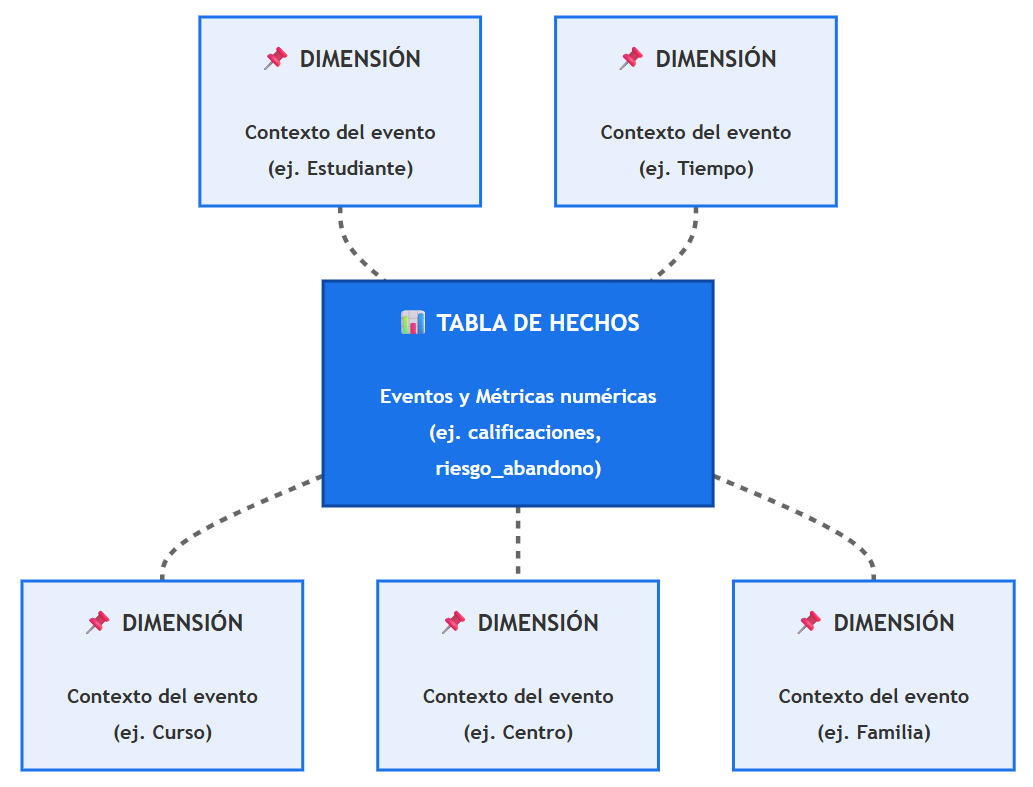
\includegraphics[width=0.8\textwidth]{imaxes/star_schema.png}
    \caption{Esquema conceptual de un modelo en estrella.}
    \label{fig:star_schema_concept}
\end{figure}

\subsection{Visualización de datos y cuadros de mando}
El objetivo final de cualquier arquitectura de Inteligencia de Negocios es la correcta comunicación de los hallazgos a los responsables de la toma de decisiones. Teóricamente, un \textit{Dashboard} o Cuadro de Mando Integral es una interfaz visual que proporciona un resumen centralizado de los Indicadores Clave de Rendimiento (de inglés KPIs). El estado del arte en el diseño de estas interfaces aboga por principios de "carga cognitiva reducida", priorizando la legibilidad, el uso de jerarquías de información y el empleo estratégico del color para señalar desviaciones críticas. Además, es fundamental la capacidad de \textit{drill-down} (profundización analítica), que permite al gestor público navegar de forma fluida desde una visión macroscópica a nivel de toda la comunidad o municipio, hasta diseccionar el estado de vulnerabilidad de un centro educativo específico.

\section{Procesos ETL y Apache Hop}
Los procesos ETL (Extracción, Transformación y Carga) son el motor de cualquier sistema BI. Son los encargados de extraer los datos de las fuentes originales, aplicarles reglas de limpieza, filtrado y transformación, y finalmente cargarlos en el Datamart dimensional.

\subsection{Elección de Apache Hop}
Apache Hop (\textit{Hop orchestration platform}) \cite{Apache_Hop} es una plataforma moderna de ingeniería de datos y orquestación. Nace como una bifurcación (\textit{fork}) de Pentaho Data Integration (PDI), con el objetivo de modernizar su arquitectura, mejorar su integración con entornos de contenedores y facilitar su uso a través de una interfaz de usuario web (\textit{Hop Web}).

La elección de Apache Hop frente a otras herramientas del mercado se fundamenta en su curva de aprendizaje, su modelo visual \textit{drag-and-drop} (ver Figura \ref{fig:apache_hop_ui}) y, especialmente, su excelente soporte para la ejecución nativa en contenedores Docker, lo cual encaja perfectamente con la arquitectura diseñada para este proyecto.

\begin{figure}[htbp]
    \centering
    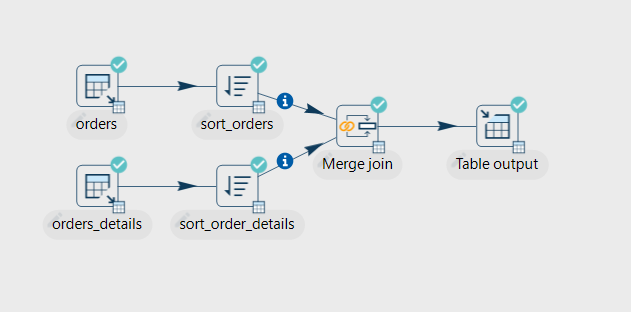
\includegraphics[width=1\textwidth]{imaxes/apache_hop_ui.png}
    \caption{Interfaz de usuario de Apache Hop.}
    \label{fig:apache_hop_ui}
\end{figure}

\section{Arquitecturas web: cliente-servidor y APIs REST}
El diseño de aplicaciones analíticas modernas ha abandonado los modelos donde el servidor generaba directamente las vistas que el usuario consumía. El marco teórico actual se fundamenta en el paradigma \textbf{Cliente-Servidor desacoplado}. En este modelo, el \textit{Frontend} (interfaz de usuario) y el \textit{Backend} (lógica de negocio y base de datos) operan como aplicaciones completamente independientes.

Para lograr la comunicación entre ambas capas, el estándar universal son las \textbf{APIs RESTful} (\textit{Representational State Transfer}). Una API REST es una interfaz que utiliza el protocolo HTTP para solicitar y enviar datos. Bajo este enfoque, el servidor expone \textit{endpoints} a los que el cliente realiza peticiones para obtener la información. Las respuestas se estructuran habitualmente en formato JSON (\textit{JavaScript Object Notation}), un estándar ligero que permite al \textit{Frontend} procesar ágilmente los datos y renderizarlos en gráficos interactivos. Este desacoplamiento es esencial para asegurar la escalabilidad del sistema.

\section{Evolución de las arquitecturas: contenedores}
El estado del arte en el despliegue de infraestructuras de datos ha sufrido un cambio de paradigma radical en los últimos años. Tradicionalmente, proyectos complejos que involucraban múltiples bases de datos, flujos ETL y servidores web se desplegaban como arquitecturas monolíticas o empleaban máquinas virtuales que consumían ingentes recursos del sistema operativo anfitrión.

La introducción de la \textbf{contenedorización}, abanderada por plataformas como Docker, representa el estándar actual de la industria. Teóricamente, un contenedor encapsula un microservicio individual junto con todas sus librerías y archivos de configuración, aislándolo completamente. Esta filosofía de "aislamiento de procesos ligeros" garantiza la inmutabilidad del software (eliminando el clásico problema de diferencias entre entornos de desarrollo y producción). Para un ecosistema educativo, donde la infraestructura tecnológica de los colegios puede ser muy limitada y heterogénea, apoyarse en este marco teórico es indispensable para asegurar un despliegue reproducible, ágil e independiente del hardware subyacente.
